\chapter{Przygotowanie środowiska - automatyzacja}

Rozpoznanie numeru autobusu, ze względu na niewielką moc obliczeniową
urządzeń mobilnych, wymagć będzie zastosowania algorytmu składającego się
z~co najmniej kilku kroków. Kolejne stopnie kaskady uszeregowane powinny 
być w~taki sposób, aby operując na dużych zbiorach danych - np.: pełne 
klatki z~kamery w~wysokich rozdzielczościach - używać algorytmów o~możliwie
najniższej złożoności obliczeniowej celem zawężenia pola poszukiwań.
Postępująca segmentacja obrazu miałaby umożliwić rozpoznanie
numeru autobusu w~czasie rzeczywistym, nie zależnie od klasy urządzenia.

Biorąc pod uwagę powyższe wymagania pierwszym krokiem (założenie robocze)
algorytmu powinna być segmentacja obrazu poprzez wykorzystanie kaskadowego
detektora haara lub LBP (powinny być opisane w~części teoretycznej).
Ze względu na różnice pomiędzy tymi dwoma detektorami pierwszym
doświadczeniem wykonanym na potrzeby tego opracowania będzie porównanie
ich wydajności i~dokładności. 

Sam proces uczenia detektorów jest jednak przedsięwzięciem żmudnym.
Dodatkowo wymaga on dużych zbiorów danych uczących oraz zbioru testowego.
W~następnych podrozdziałach przedstawione zostaną narzędzia których
zadaniem będzie maksymalna automatyzacja i~optymalizacja procesu uczenia
oraz weryfikacji zarówno skuteczności jak i~wydajności uzyskanych wersji
detektorów.

Oczywiście w~dalszych podrozdziałach opisane zostaną kolejne robocze
kroki algorytmu, a~także narzędzia służące w~ich przygotowaniu oraz 
weryfikacji.

Celem tego rozdziału jest więc udokumentowanie doświadczeń przeprowadzonych
na drodze do osiągnięcia optymalnego algorytmu rozpoznawania numeru
autobusu.

\section{Wspomaganie pobierania filmów z serwisu YouTube}

Pewnego rodzaju rozgrzewką było przygotowanie wtyczki do przeglądarki 
Firefox ułatwiającej pobieranie i wstępne katalogowanie filmów
udostępnianych za pośrednictwem serwisu YouTube.

Założenia oraz oczekiwania funkcjonalne wobec omawianego narzędzia były 
następujące:

\begin{enumerate}
    \item Wizualizacja stanu w~jakim znajduje się oglądany film - 
        możliwe są dwa stany:
    \begin{itemize}
        \item co najmniej jedna wersja filmu została już pobrana,
        \item film nie został pobrany w~żadnej wersji.
    \end{itemize}
    \item Możliwość pobrania wybranej wersji filmu w~odległości maksymalnie
        dwuch kliknięć licząc od poziomu przeglądania filmów w~serwisie,
    \item Tworzenie pliku CSV (\textit{ang. Comma Separated Value})
        z~danymi pobranych filmów, celem identyfikacji już pobranych
        pozycji. Plik powinien być tak skonstruowany aby można go było
        również wykorzystać do odtworzenia bazy filmów na dysku. W~razie
        awarii lub chęci przeprowadzenia całego procesu uczenia od
        początku.
\end{enumerate}

\subsection{Pierwsza wersja wtyczki - stan}

Przedstawienie stanu aktualnie oglądanego filmu odbywa się poprzez
kolor dodatkowej ikony wkomponowanej w~lewe pionowe menu, zaraz obok
wyświetlanego filmu.

\begin{figure}[h!]
    \caption{Przycisk rozwijanego menu, oraz wskaźnik stanu}
    \centering
    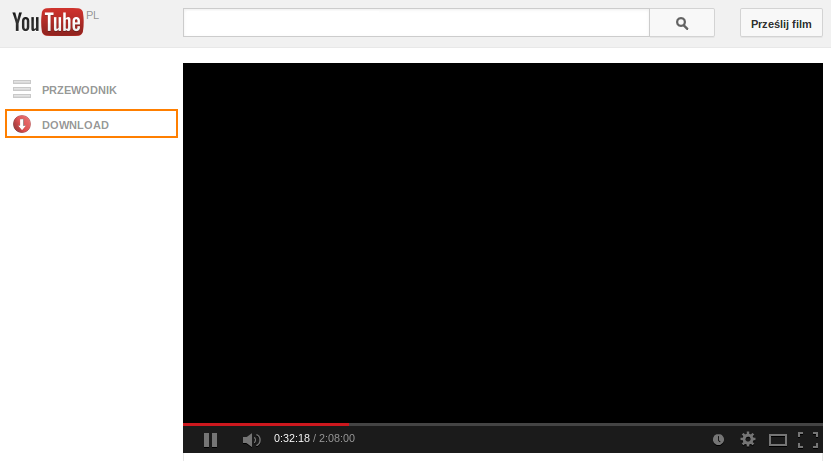
\includegraphics[width=0.9\textwidth]{img/env_yt_dwn_indicator}
\end{figure}

Kolor czerwony wskazuje, że oglądany film nie został jeszcze pobrany.
Ikona z~pustą strzałką w~środku w~kolorze zielonym sygnalizuje obecność
oglądanej pozycji w~wyżej wymienionym pliku rozdzielanym przecinkami
(pkt. 3).

Postępy w~pracach nad pierwszą wersją wtyczki doprowadziły do wypełnienia
założeń funkcjonalnych przez ostatnią wersję programu. Koncepcja wkomponowania
menu w~treść strony, oraz funkcjonalność pobierania filmów okazały się
na tyle problematyczne i~trudno zarządzalne, że powstała druga wersja programu
o~znacznie ograniczonej funkcjonalności.

\subsection{Druga wersja wtyczki - funkcjonalność}

Funkcjonalność drugiej wersji programu została ograniczona do minimum. Faktycznie
ograniczała się ona do oznaczania wybranego filmu wraz z~jego wersją, oraz
eksportu tak utworzonych wpisów do pliku - id filmu oraz numer identyfikacyjny wersji.

Przepływ sterowania dla drugiej wersji programu został przedstawiony na poniższym
diagramie. Funkcja implementująca pokazany algorytm jest wywoływana za każdym razem
gdy zmieni się wartość url-a w~aktywnej karcie przeglądarki lub kliknięty zostanie
któryś z~przycisków w stanach ,,żółtym'' lub ,,zielonym''.

\begin{figure}[h!]
    \caption{Algorytm aktualizacji stanu wtyczki w wersji drugiej}
    \centering
    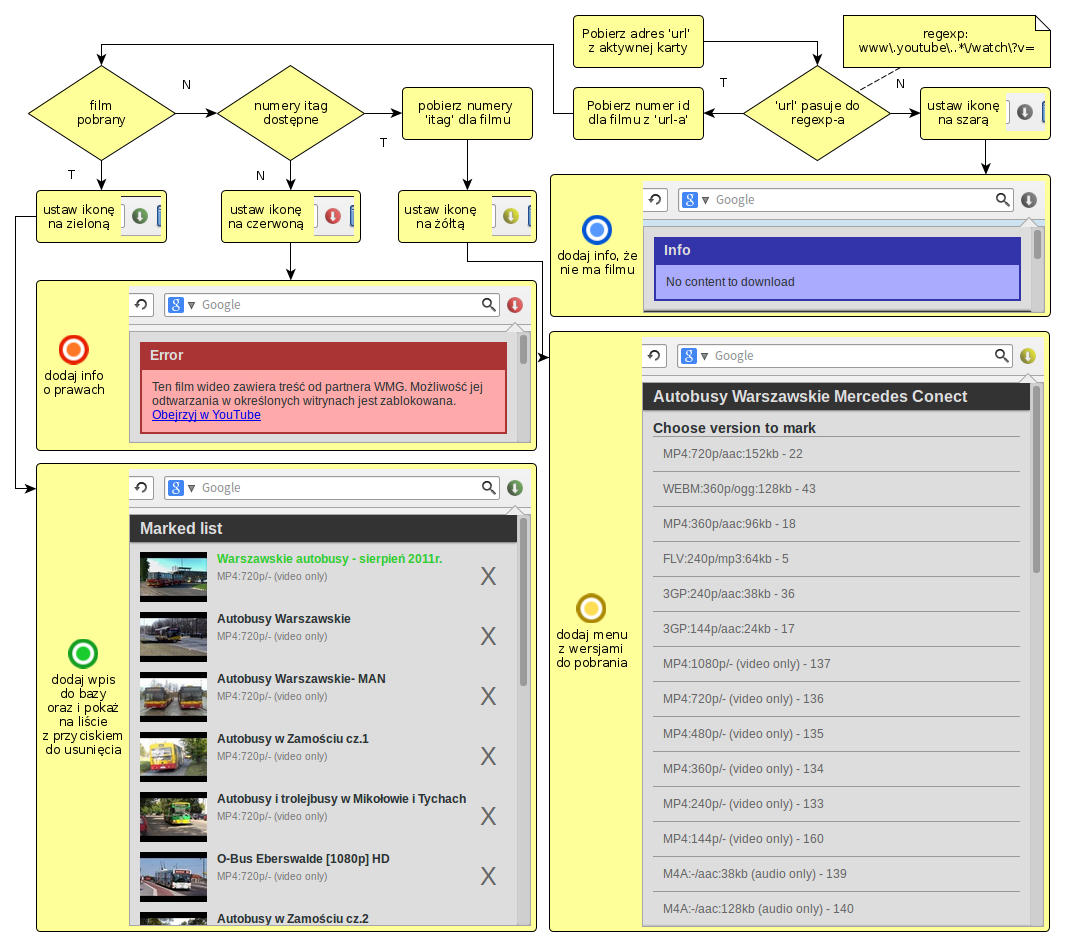
\includegraphics[width=0.9\textwidth]{img/env_yt_marker}
\end{figure}

Niestety program pierwszy program ,,pomocniczy'' okazał się narzędziem nie adekwatnym
(zbyt skomplikowanym i~pracochłonnym) do postawionego mu zadania. Okazało się, że
filmów zawierających fronty autobusów jest znacznie mniej niż mogło by się wydawać.

Po znalezieniu 14 pozycji zawartość serwisu (odnośnie frontów autobusów) nagle się
wyczerpała. Ostatecznie wielotygodniowe (dokładnie dwu) prace nad wtyczką do programu 
Firefox zaowocowały bazą czternastu pozycji w~formie pliku CSV zawierającego dwie
kolumny:

\begin{itemize}
    \item id filmu, np.: 75Dz6s7S-Tg;
    \item itag reprezentujący wybraną wersję, np.: 136
\end{itemize}

W~naszym przypadku wszystkie filmy zostały ,,oznaczone'' w~wersji 136, czyli
zawierającej tylko obraz, oraz będącej w~rozdzielczośći HD (720p).

Ostatecznie owoc pracy przedstawiony jest poniżej.

\lstinputlisting{../data/description_files/marked_for_download/yt_marked_01.csv}

Co niestety o~wiele szybciej, prościej, wydajniej, taniej i~krótko mówiąc lepiej można
by wykonać bez implementowania żadnych narzędzi. Jedyne co pozostało to zdobyta wiedza
na temat: javascript, css, html, firefox: xul, addon-sdk, cfx. 

Kolejne narzędzia ,,pomocnicze'' implementowane będą z~większą ostrożnością i~po
dłuższym przeanalizowaniu zagadnienia poddawanego automatyzacji.


